\documentclass[a4paper, 12pt]{article}%тип документа



%отступы
\usepackage[left=1cm,right=1cm,top=1cm,bottom=2cm,bindingoffset=0cm]{geometry}

%%% Работа с русским языком
\usepackage{graphicx}
\usepackage{cmap}                           % поиск в PDF
\usepackage{mathtext} 			 	       % русские буквы в формулах
\usepackage[T2A]{fontenc}               % кодировка
\usepackage[utf8]{inputenc}              % кодировка исходного текста
\usepackage[english,russian]{babel} 
\usepackage{float}

\usepackage[export]{adjustbox} % локализация и переносы

\usepackage{subfig}% http://ctan.org/pkg/subfig
\usepackage{booktabs}

\usepackage{wrapfig}


%Матеша
\usepackage{amsmath,amsfonts,amssymb,amsthm,mathtools} % AMS
\usepackage{icomma} % "Умная" запятая

%\mathtoolsset{showonlyrefs=true} % Показывать номера только у тех формул, на которые есть \eqref{} в тексте.

%% Шрифты
\usepackage{euscript}	 % Шрифт Евклид
\usepackage{mathrsfs} % Красивый матшрифт

%% Свои команды
\DeclareMathOperator{\sgn}{\mathop{sgn}}

%% Перенос знаков в формулах (по Львовскому)
\newcommand*{\hm}[1]{#1\nobreak\discretionary{}
	{\hbox{$\mathsurround=0pt #1$}}{}}


%\usepackage{caption}
%\usepackage{subcaption}


\author{Гаврилин Илья Дмитриевич \\
	Б01-101}
\title{\textbf{Работа 3.6.1 \\ 
		Исследование спектра колебаний электрических сигналов}}

\begin{document}
	\maketitle
	\section{Аннотация}
	В данной работе изучили принцип работы осциллографа с быстрым преобразованием Фурье, рассмотрели спектры прямоугольного сигнала, цугов, частотно и амплитудно модулированного сигнала. Рассмотрели как изменится спектр при изменении параметров сигнала.
	\section{Теоретические сведения}
	\subsection*{Разложение сложных сигналов на периодические колебания}
	Используется разложение в сумму синусов и косинусов с различными аргументами или, как чаще его называют, \textit{разложение в ряд Фурье}.
	
	Пусть задана функция $f(t)$, которая периодически повторяется с частотой $\Omega_1 = \dfrac{2\pi}{T}$, где $T$ --- период повторения импульсов. Её разложение в ряд Фурье имеет вид 
	\begin{equation}
		f(t) = \dfrac{a_0}{2} + \sum\limits_{n = 1}^{\infty}\left[a_n \cos \left(n \Omega_1t\right) + b_n \sin \left(n \Omega_1t\right)\right]
	\end{equation}
	или
	\begin{equation}
		f(t) = \dfrac{a_0}{2} + \sum\limits_{n = 1}^{\infty}A_n \cos \left(n\Omega_1t-\psi_n\right).
	\end{equation}
	Если сигнал чётен относительно $t=0$, в тригонометрической записи остаются только члены с косинусами. Для нечетной наоборот.
	
	Коэффициенты определяются по формуле
	\begin{equation}
		\begin{array}{c}
			a_n  = \dfrac{2}{T}\int\limits_{t_1}^{t_1+T}f(t)\cos\left(n \Omega_1 t\right) dt,\\
			\\
			b_n = \dfrac{2}{T}\int\limits_{t_1}^{t_1+T}f(t)\sin\left(n \Omega_1 t\right) dt.
		\end{array}
	\end{equation}
	Здесь $t_1$ --- время, с которого мы начинаем отсчет.
	
	Сравнив формулы $(1)$ и $(2)$ можно получить выражения для $A_n$  и $\psi_n$:
	\begin{equation}
		\begin{array}{l}
			A_n = \sqrt{a_n^2+b_n^2},\\
			\psi_n = \arctan \dfrac{b_n}{a_n}.
		\end{array}
	\end{equation}
	\subsection*{Периодическая последовательность прямоугольных импульсов}
	Введем величину: $\Omega_1 = \dfrac{2\pi}{T}$,
	где $T$ --- период повторения импульсов.
	
	Коэффициенты при косинусных составляющих будут равны
	\begin{equation}
		a_n = \dfrac{2}{T}\int\limits_{-\tau/2}^{\tau/2}V_0\cos\left(n\Omega_1 t\right)dt = 2V_0\dfrac{\tau}{T}\dfrac{\sin\left(n\Omega_1\tau/2\right)}{n\Omega_1\tau/2} \sim \dfrac{\sin x}{x}.
	\end{equation}
	
	Здесь $V_0$ - амплитуда сигнала.
	
	Поскольку наша функция четная, то $b_n = 0$. 
	
	Пусть $T$ кратно $\tau$. Тогда введем ширину спектра, равную $\Delta \omega$ --- расстояние от главного максимума до первого нуля огибающей, возникающего, как нетрудно убедиться при $n = \dfrac{2\pi}{\tau \Omega_1}$. При 
	этом
	\begin{equation}
		\Delta \omega \tau \simeq 2\pi \Rightarrow \Delta \nu \Delta t \simeq 1.
	\end{equation}
	\subsection*{Периодическая последовательность цугов}
	Возьмём цуги колебания $V_0 \cos(\omega_0 t)$ с длительностью цуга $\tau$ и периодом повторений $T$.\\
	Функция $f(t)$ снова является четной относительно $t = 0$. Коэффициент при $n$-ой гармонике согласно формуле $(3)$ равен
	\begin{equation}
		a_n = \dfrac{2}{T}\int\limits_{-\tau/2}^{\tau/2}V_0 \cos \left(\omega_0t\right) \cdot \cos\left(n \Omega_1t\right)dt = V_0 \dfrac{\tau}{T}\left( \dfrac{\sin\left[\left(\omega_0 - n \Omega_1\right)\dfrac{\tau}{2}\right]}{\left( \omega_0 - n \Omega_1\right) \dfrac{\tau}{2}} + \dfrac{\sin\left[\left(\omega_0 + n \Omega_1\right)\dfrac{\tau}{2}\right]}{\left( \omega_0 + n \Omega_1\right) \dfrac{\tau}{2}}\right).
	\end{equation}
	Пусть $T$ кратно $\tau$. Тогда спектры последовательности прямоугольных сигналов и цугов аналогичны, но максимумы сдвинуты на $\omega_0$.
	\subsection*{Амплитудно-модулированные колебания}
	
	Рассмотрим гармонические колебания высокой частоты $\omega_0$, амплитуда которых медленно меняется по гармоническому закону с частотой $\Omega \ll \omega_0$.
	\begin{equation}
		f(t) = A_0 \left[1+m\cos \Omega t\right] \cos \omega_0 t.
	\end{equation}
	Коэффициент $m$ называется \textit{глубиной модуляции}. При $m < 1$ амплитуда меняется от минимальной $A_{min} = A_0(1-m)$ до максимальной $A_{max} = A_0(1+m)$. Глубина модуляции может быть представлена в виде
	\begin{equation}
		m = \dfrac{A_{max}-A_{min}}{A_{max}+A_{min}}.
	\end{equation}
	Простым тригонометрическим преобразованием уравнения $(8)$ можно найти спектр колебаний
	\begin{equation}
		f(t) = A_0 \cos \omega_0t + \dfrac{A_0m}{2} \cos \left(\omega_0 + \Omega\right)t + \dfrac{A_0m}{2}\cos\left(\omega_0 - \Omega\right)t.
	\end{equation}
	
	\section{Ход работы}
	\subsection{Исследование спектра периодических последовательностей прямоугольных импульсов}
	Устанавливаем прямоугольные колебания c $\nu_{повт} = 1$ кГц (период $T = 1$ мс) и длительностью импульса $\tau = T/20 = 50$ мкс.
	
	Получаем на экране спектр сигнала и, изменяя либо $\tau$, либо $\nu_{повт}$, наблюдаем, как изменяется спектр.
	\begin{figure}[H]
		\centering
		\subfloat[$\nu_{повт} = 1$ кГц, $\tau = 50$ мкс.]{{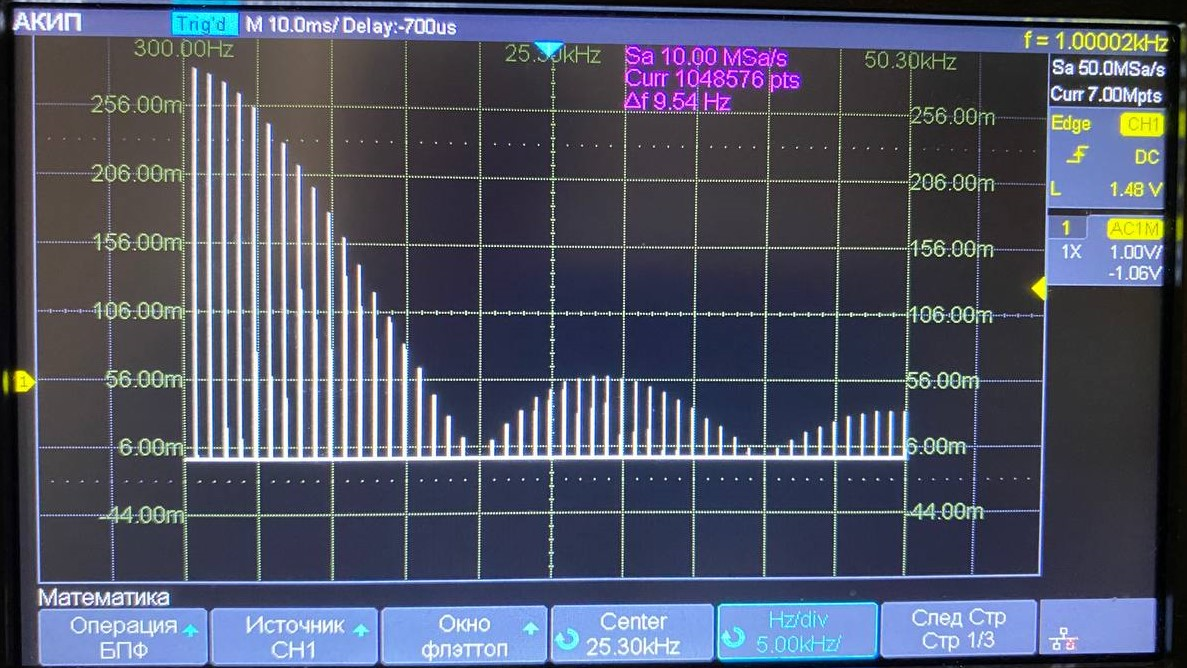
\includegraphics[width=0.8\textwidth]{photo_1.jpg}}}\\
		\subfloat[$\nu_{повт} = 1.5$ кГц, $\tau = 25$ мкс.]{{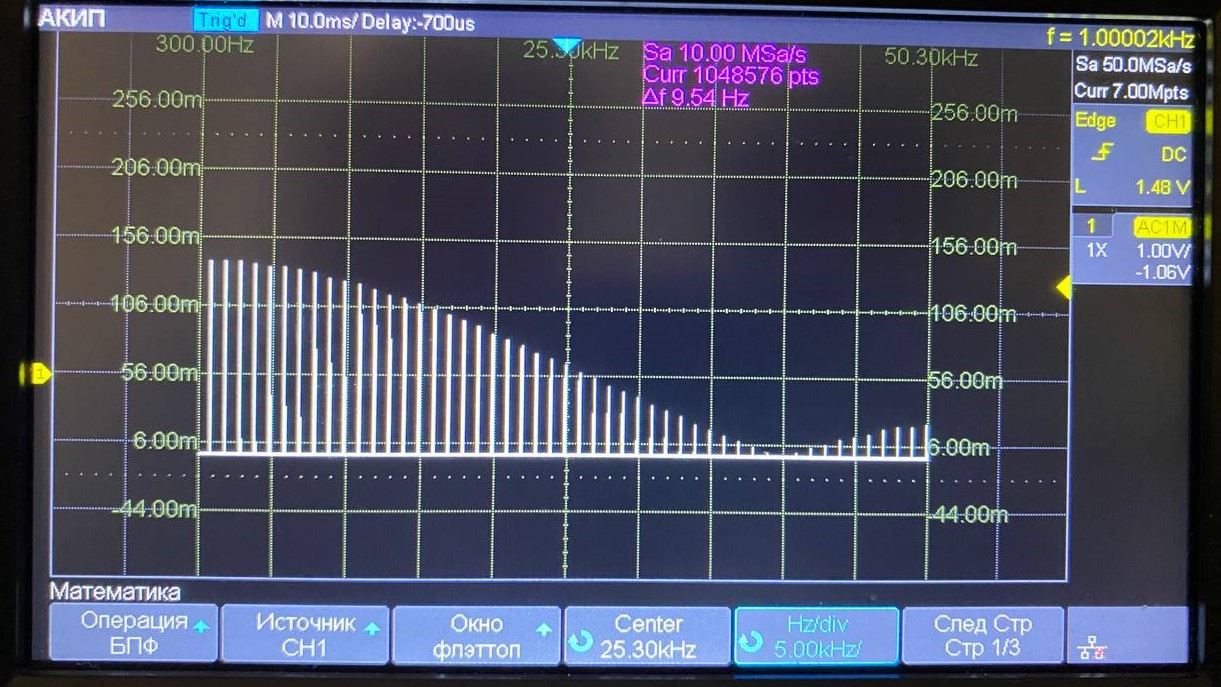
\includegraphics[width=0.478\textwidth]{photo_2.jpg}}}
		\qquad
		\subfloat[$\nu_{повт} = 2$ кГц, $\tau = 50$ мкс.]{{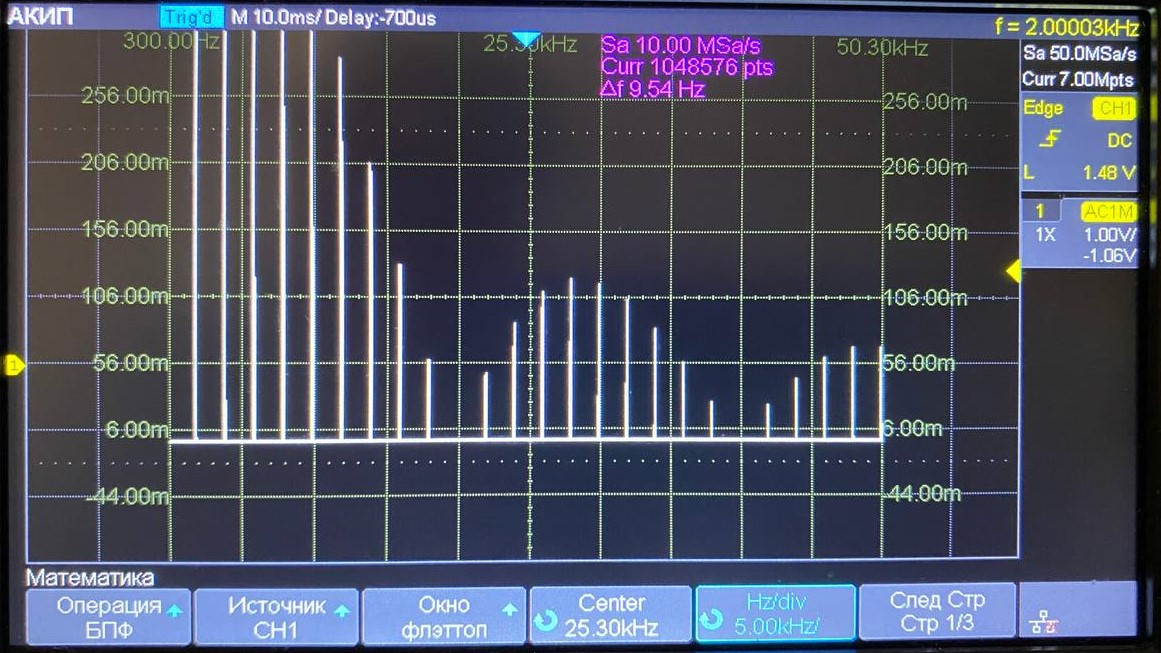
\includegraphics[width=0.478\textwidth]{photo_3.jpg}}}
		\caption{Спектры периодических последовательностей прямоугольных импульсов}
	\end{figure}
	Рассмотрим как меняется спектр при изменении параметров относительно начального спектра (Рис. 1(а)).\\
	Заметим что при уменьшении $\tau$ в 2 раза: ширина спектра увеличивается в 2 раза, расстояние между гармониками не меняется, количество гармоник увеличивается в 2 раза (Рис. 1(b)).\\
	При увеличении $\nu_{повт}$ в 2 раза: ширина спектра не меняется, расстояние между гармониками увеличивается в 2 раза, количество гармоник уменьшается в 2 раза(Рис. 1(c)).\\
	Рассмотрим связь амплитуды конкретной гармоники с ее частотой. Предложенная в работе формула (6.12)\footnote{см. Лабораторный практикум по общей физике Том 2 электричество и магнетизм, МФТИ, страница 293} предусматривает рассчет для зависимости спектра в комплексном представлении от циклической частоты. В работе же получили связь действительного спектра по частотам. Однако, мы знаем что спектр эквивалентен $ \propto |\frac{sin(x)}{x}| $, используя это предположение проверим верность полученного спектра.
	\begin{table}[H]
		\centering
		\begin{tabular}{|c|c|c|}
			\hline
			\multicolumn{1}{|l|}{№ гармоники} & \multicolumn{1}{l|}{$\nu$, kГц} & \multicolumn{1}{l|}{$a_n$, мВ} \\ \hline
			1                           & 1.02                        & 288                          \\ \hline
			2                           & 2.10                        & 222                          \\ \hline
			3                           & 3.06                        & 219                          \\ \hline
			4                           & 4.02                        & 210                          \\ \hline
			5                           & 5.02                        & 204                          \\ \hline
			6                           & 5.98                        & 196      \\ \hline                   
		\end{tabular}
		\caption{Связь частоты и амплитуды первых 6-ти гармоник для прямоугольного сигнала}
	\end{table}
	\begin{figure}[H]
		\centering
		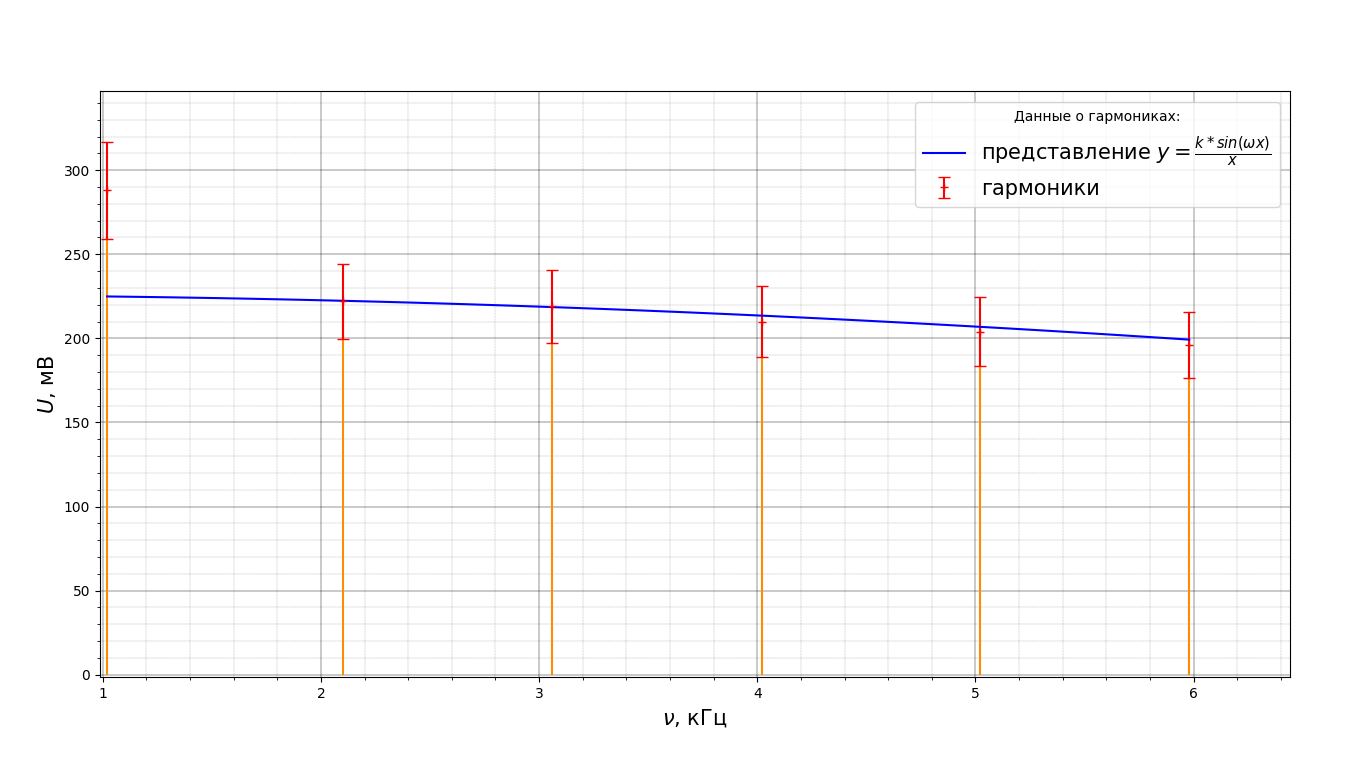
\includegraphics[width=0.9\linewidth]{прямоуг}
		\caption{наложение графика $|\frac{sin(x)}{x}|$ на первые гармоники прямоугольного сигнала}
		\label{fig:}
	\end{figure}
	Как мы можем видеть первые гармоники, за исключением быть может первой, ложатся на теоретическую кривую, что означает справедливость теоретических соображений. Для остальных точек совпадение с данной кривой можно заметить визуально, взглянув на Рис. 1(а).\\
	Проверим справедливость формулы (6). Для этого снимем 5 различный значений $\tau$ и $\Delta \nu$, по итогу должны получить зависимость $\Delta \nu \cdot \tau = 1$.
	\begin{table}[H]
		\centering
		\begin{tabular}{|l|c|c|c|c|c|}
			\hline
			$\tau$, мкс        & 20.00   & 60.00   & 100.00&  140.00 & 180.00 \\ \hline
			$\Delta \nu$, kГц & 48.0 & 15.8 & 9.0 & 6.0 & 4.8 \\ \hline
		\end{tabular}
	\caption{Значения $\Delta \nu$ и $\tau$ для прямоугольного сигнала}
	\end{table}
	Оценим погрешность как:\\
	для $\tau$ возьмем как последний разряд показывающийся на генераторе сигнала $\delta \tau = \pm 0.01$ мкс;\\
	для $\Delta \nu$ возьмем в качестве погрешности половину наименьшего деления  осциллографа $\delta \Delta \nu = \pm 0.5$ кГц;\\
	Для Рис.2 данные оценки погрешности также справедливы.
	\begin{figure}[H]
		\centering
		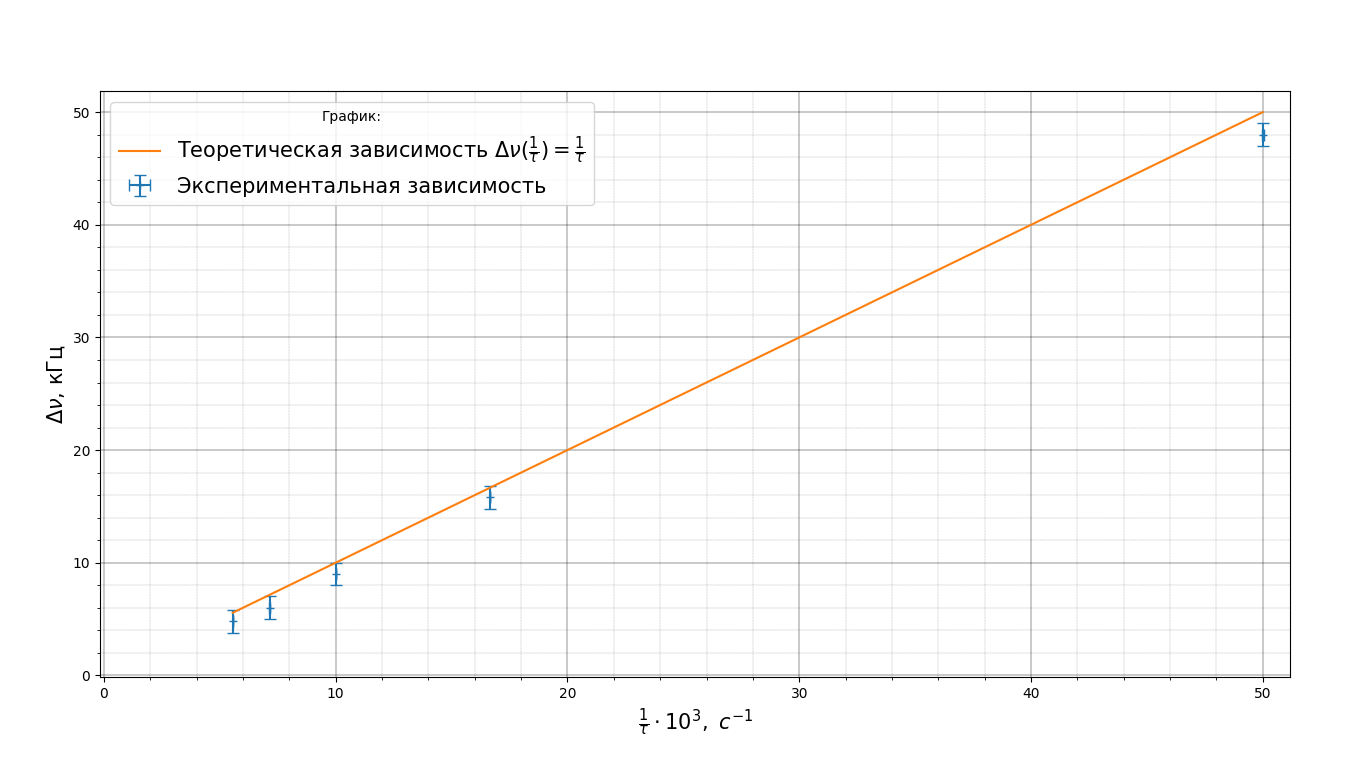
\includegraphics[width=0.9\linewidth]{завис_1}
		\caption{Зависимость $\Delta \nu(\frac{1}{\tau}) = \frac{1}{\tau}$ для прямоугольного сигнала}
		\label{fig:1}
	\end{figure}
	\subsection{Исследование спектра периодической последовательности цугов}
	 Получаем на экране последовательность цугов с характерными параметрами: $\nu_0 = 50$ кГц, $T = 1$ мс, число периодов в одном импульсе $N = 5$ (длительность импульса $\tau = T/\nu_0 = 100$ мкс).
	 \begin{figure}[H]
	 	\centering
	 	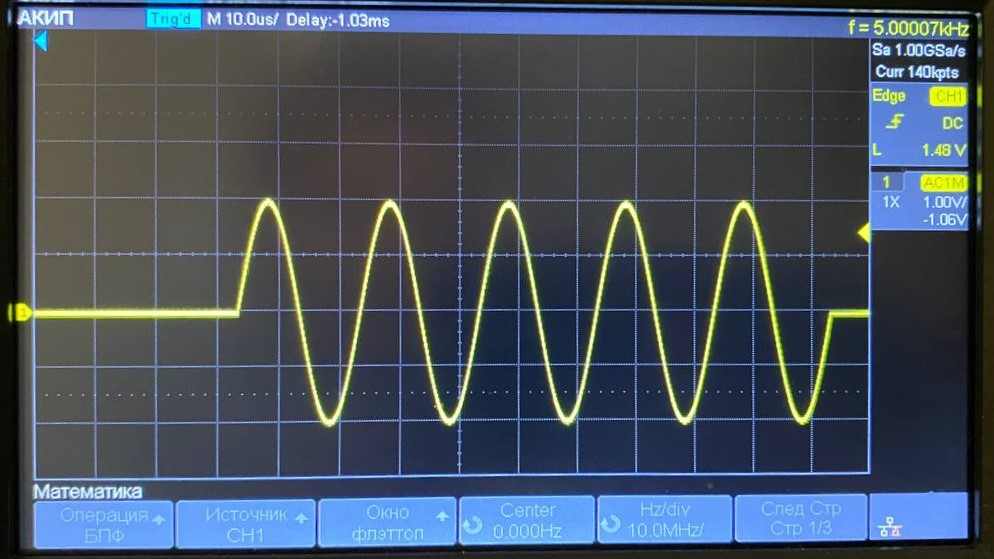
\includegraphics[width=0.9\linewidth]{photo_4}
	 	\caption{Осциллограмма последовательности цугов}
	 	\label{fig:photo4}
	 \end{figure}
	 Теперь будем менять эти параметры по одному и зафиксируем несколько таких изменений:
	 \begin{figure}[H]
	 	\centering
	 	\subfloat[$\nu_0 = 50$ кГц, $T = 1$ мс, $N = 10$ ]{{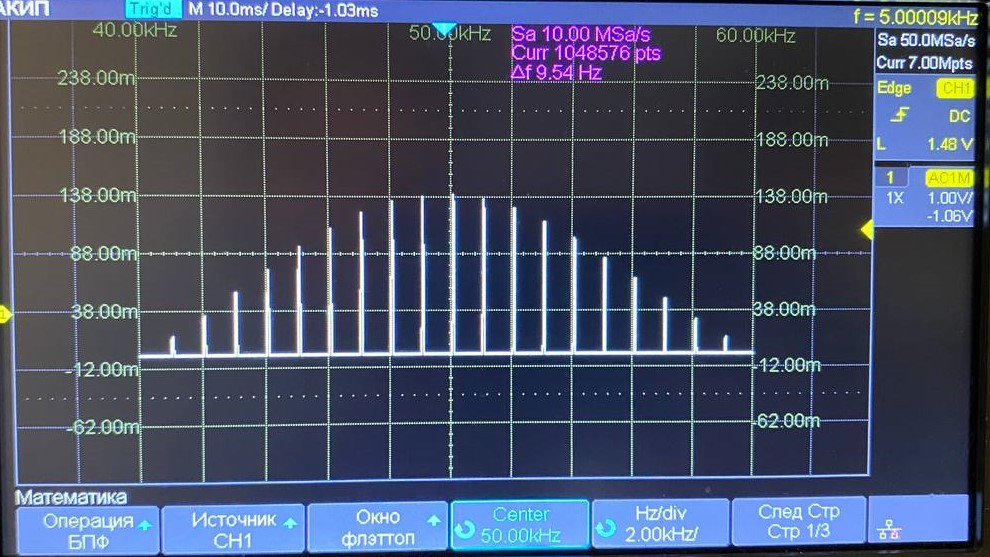
\includegraphics[width=0.478\textwidth]{photo_5.jpg}}}
	 	\qquad
	 	\subfloat[$\nu_0 = 100$ кГц, $T = 1$ мс, $N = 10$ ]{{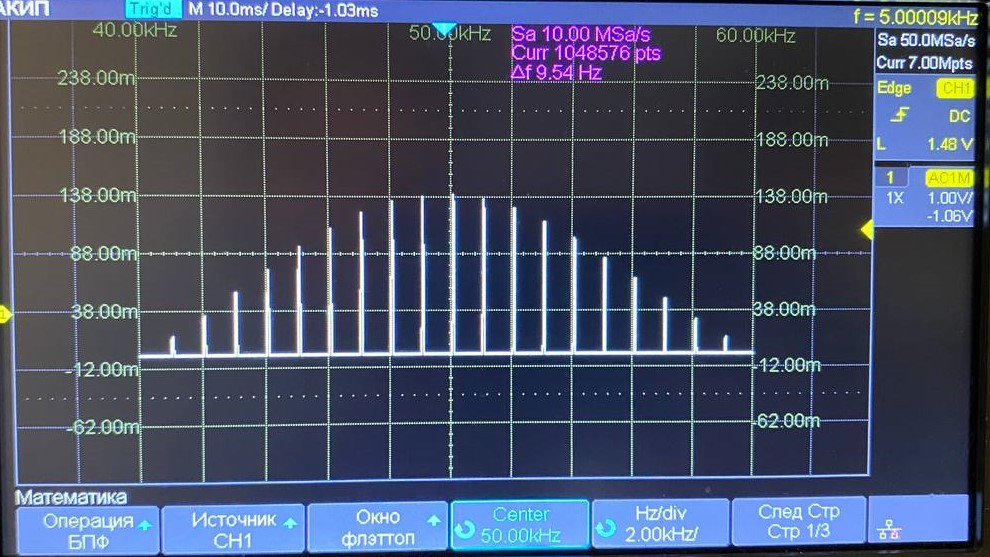
\includegraphics[width=0.478\textwidth]{photo_5.jpg}}}\\
	 	\subfloat[$\nu_0 = 100$ кГц, $T = 2$ мс, $N = 10$]{{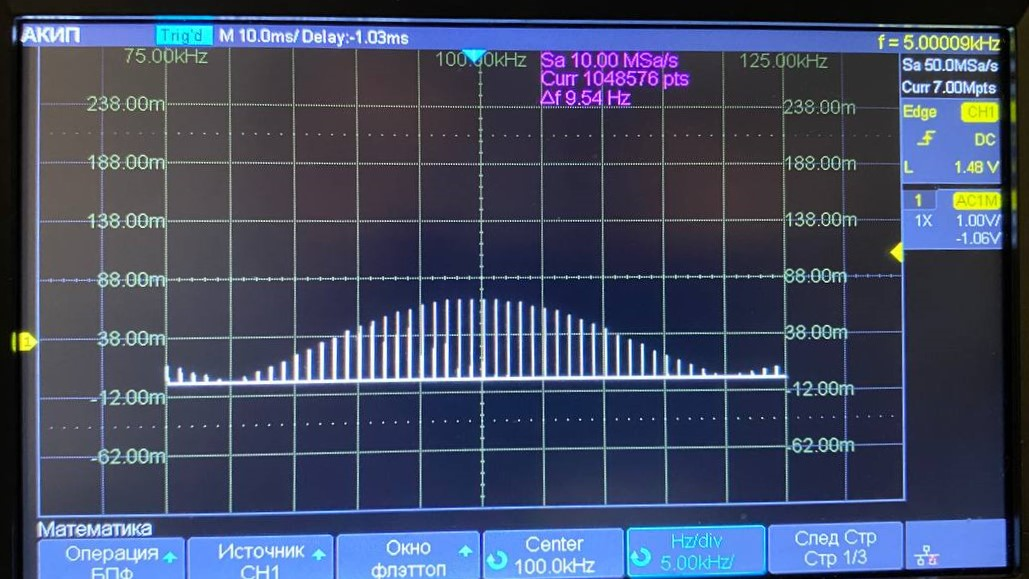
\includegraphics[width=0.478\textwidth]{photo_6.jpg}}}
	 	\qquad
	 	\subfloat[$\nu_0 = 50$ кГц, $T = 1$ мс, $N = 20$]{{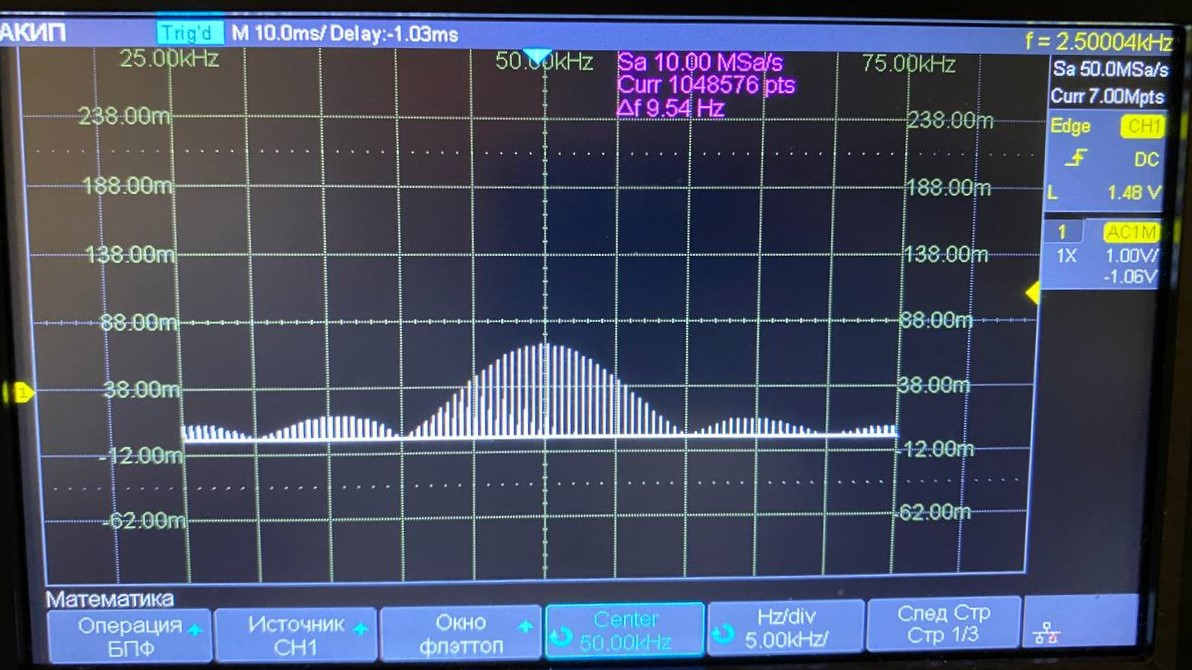
\includegraphics[width=0.478\textwidth]{photo_7.jpg}}}
	 	\caption{Спектры периодических последовательностей цугов}
	 \end{figure}
 	Рассмотрим изменение спектров при изменении основных параметров:\\
 	При увеличении $\nu_0$ в 2 раза середина сдвигается в 2 раза вправо, остальные параметры неизменны (Рис. 5(b)). \\
 	При увеличении $T$ в 2 раза $a_n$ уменьшается в 2 раза, количество гармоник увеличивается в 2 раза, расстояние между ними уменьшается в 2 раза (Рис. 5(с)). \\
 	При увеличении $N$ в 2 раза ширина спектра уменьшается в 2 раза, расстояние между гармониками уменьшается в 2 раза (Рис. 5(d)). \\
 	Теперь зафиксируем $\nu_0 = 50$ кГц, $N = 5$. Для этих параметров измерим, $T$ и  $\delta \nu$.
 	\begin{table}[H]
 		\centering
 		\begin{tabular}{|c|c|c|c|c|c|c|}
 			\hline
 			$T$, мс  & 0.2  & 1.0  & 1.5 & 2.0 & 3.0 & 5.0 \\ \hline
 			 $\delta \nu$, Гц& 5000 & 1000 & 680 & 508 & 336 & 204 \\ \hline
 		\end{tabular}
 		\caption{Связь $T$ и  $\delta \nu$ для последовательности цугов}
 	\end{table}
 	Построим зависимость $\delta \nu(\frac{1}{T})$б исходя из теории должны получить $\delta \nu(\frac{1}{T}) = \frac{1}{T}$
 	\begin{figure}[H]
 		\centering
 		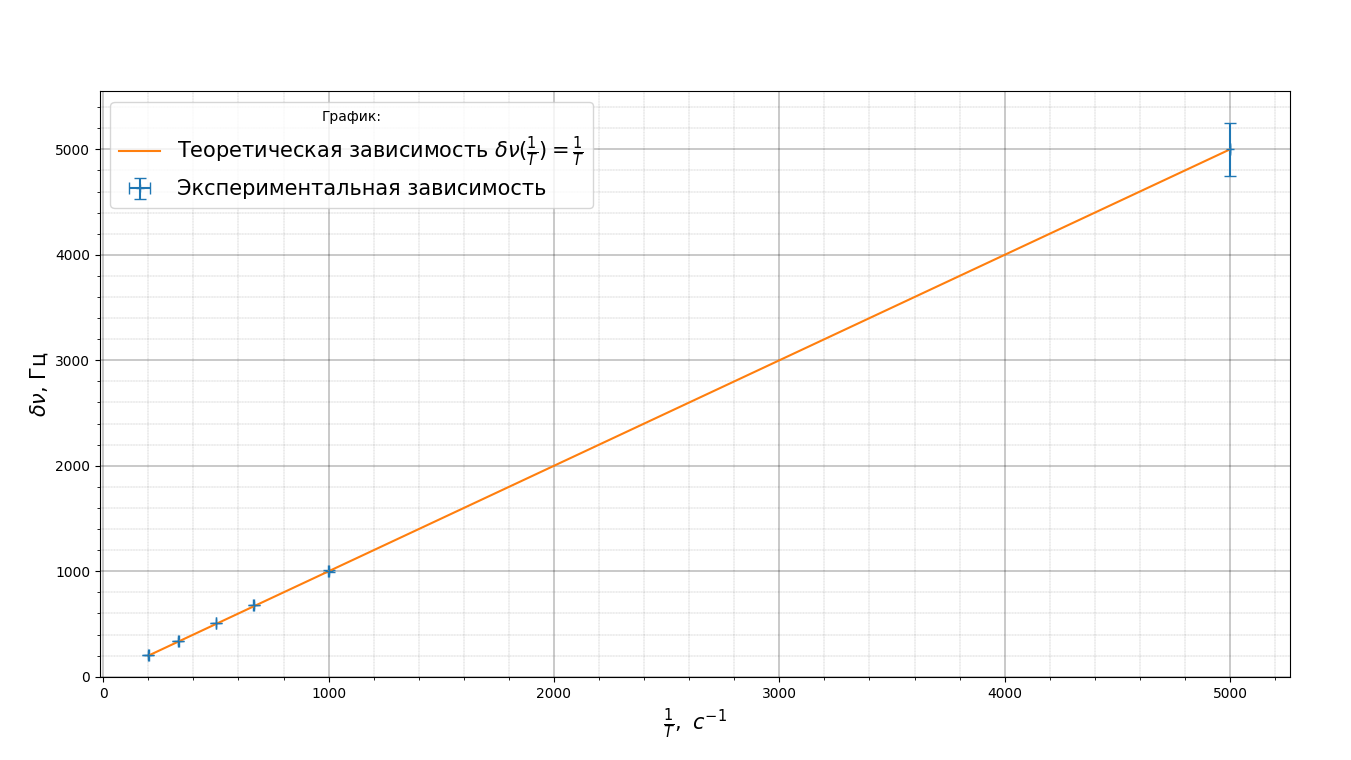
\includegraphics[width=0.9\linewidth]{завис_2}
 		\caption{Зависимость $\delta \nu(\frac{1}{T})$ для последовательности цугов}
 		\label{fig:2}
 	\end{figure}
 	Заметим что полученные нами данные совпадают с теоретическим предположением в рамках погрешности.
 	\subsection{Исследование спектра амплитудно модулированного сигнала}
 	Выведем на экран картину амплитудно-модулированного сигнала с характерными параметрами: несущая частота $\nu_0 = 50$ кГц, $\nu_{\text{мод}} = 2$ кГц, глубина модуляции - 50 \% ($m = 0.5$).\\
 	Найдем для него $A_{max}$ и $A_{min}$ и проверим справедливость формулы $(9)$.
 	\begin{center}
 		\begin{tabular}{|c|c|}
 			\hline
 			$A_{max}$, мВ & 1560 \\ \hline
 			$A_{min}$, мВ & 520 \\ \hline
 			$m$ & 0.5 \\ \hline
 		\end{tabular}
 	\end{center}
 	Получили значение полностью совпадающее с теоретической зависимостью, что может говорить о справедливости формулы (9).
 	Получим на экране спектр и будем изменять параметры сигнала:
 	\begin{figure}[H]
 		\centering
 		\subfloat[$\nu_0 = 50$ кГц, $\nu_{\text{мод}} = 2$ кГц.]{{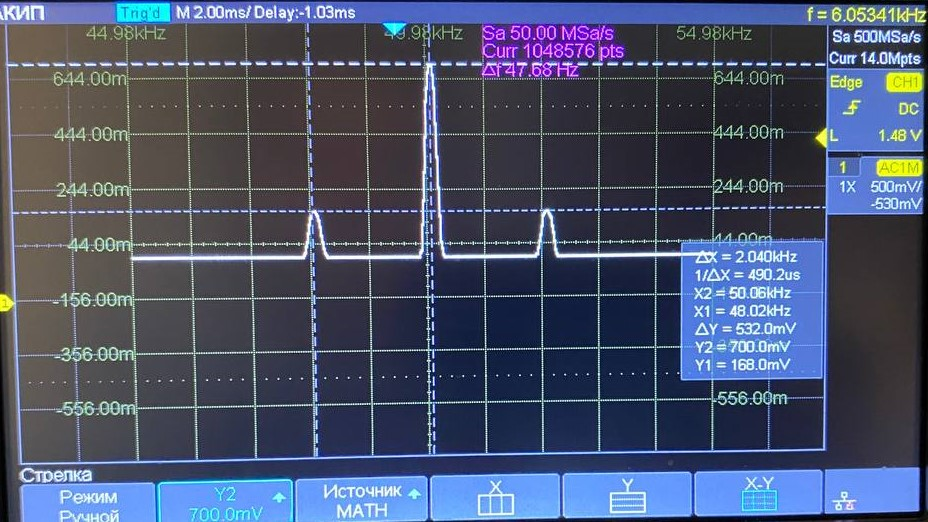
\includegraphics[width=0.478\textwidth]{photo_9.jpg}}}
 		\qquad
 		\subfloat[$\nu_0 = 100$ кГц, $\nu_{\text{мод}} = 2$ кГц.]{{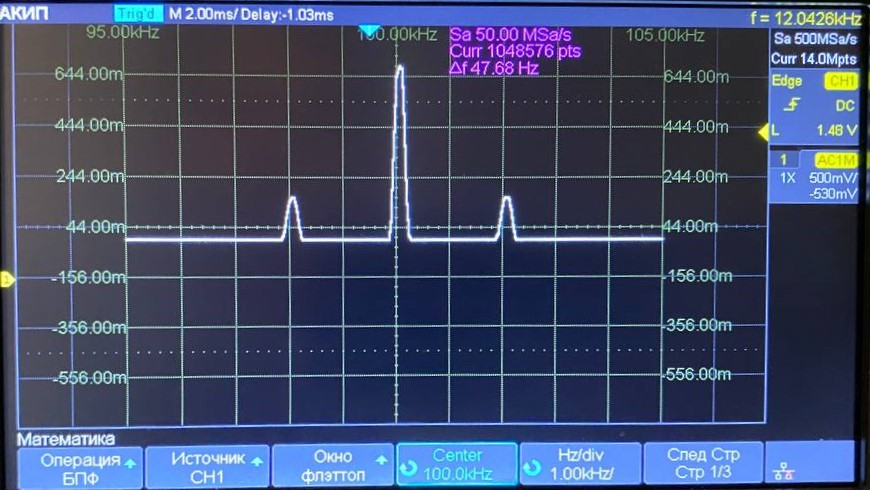
\includegraphics[width=0.478\textwidth]{photo_10.jpg}}}    		\caption{Спектр амплитудно модулированного сигнала}	
 	\end{figure}
 	Заметим что при изменении основной частоты происходит соответствующий сдвиг пика спектра, при увеличении модулирующей частоты увеличивается расстояние от основной до боковых гармоник.
 	\begin{table}[H]
 		\centering
 		\begin{tabular}{|l|c|c|c|c|c|c|}
 			\hline
 			m, \%     & 10    & 30    & 50    & 70    & 90    & 100   \\ \hline
 			$\frac{а_{бок}}{а_{осн}}$ & 0.045 & 0.153 & 0.239 & 0.347 & 0.438 & 0.490 \\ \hline
 		\end{tabular}
 		\caption{Связь m и $\frac{а_{бок}}{а_{осн}}$ для амплитудно модулированного сигнала}
 	\end{table}
 	По полученным значениям построим зависимость и сравним с теоретическим значением 1/2.
 	\begin{figure}[H]
 		\centering
 		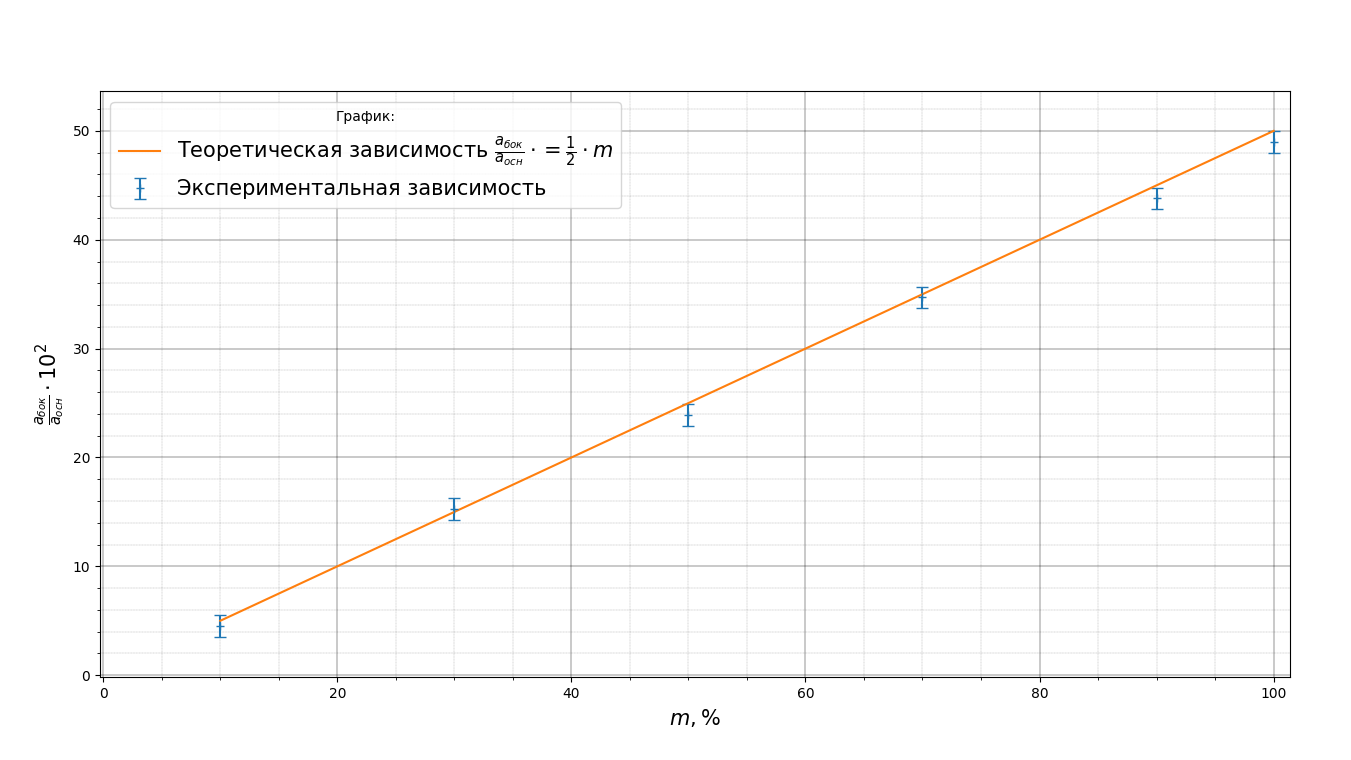
\includegraphics[width=0.9\linewidth]{завис_3}
 		\caption{Зависимость $\frac{а_{бок}}{а_{осн}}(m)$ для амплитудно модулированного сигнала}
 		\label{fig:3}
 	\end{figure}
 	\subsection{Фазово модулированный сигнал}
 	Установили на генераторе режим
 	модулированного по фазе синусоидального сигнала с несущей $\nu_0$ = 50 кГц,
 	частотой модуляции $\nu_{мод}$ = 2 кГц и максимальным отклонением (глубиной
 	модуляции) фазы $\phi_{m}$ = $10^\circ$
 	. Получите на экране осциллографа устойчивую
 	картину сигнала.
 	\begin{figure}[H]
 		\centering
 		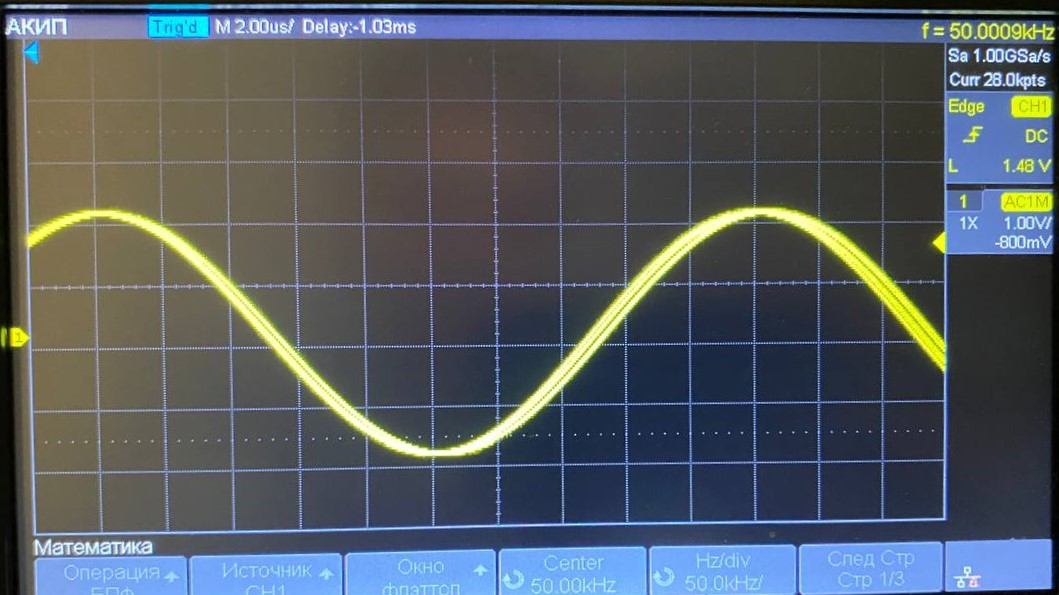
\includegraphics[width=0.7\linewidth]{photo_11}
 		\caption{Фазово модулированный сигнал}
 		\label{fig:photo11}
 	\end{figure}
 	Изменение несущей и модулирующей частоты приводит к тем же изменениям, что и для амплитудно модулированного сигнала. Изучим влияние изменения фазы сигнала.
 	Экспериментально определили что при $\phi_{m}$ = $82^\circ$ средний пик сравнивается с боковыми, а после начинает убывать.
 	\begin{figure}[H]
 		\centering
 			\subfloat[$\nu_0 = 50$ кГц, $\nu_{\text{мод}} = 2$ кГц, $\phi_{m}$ = $10^\circ$.]{{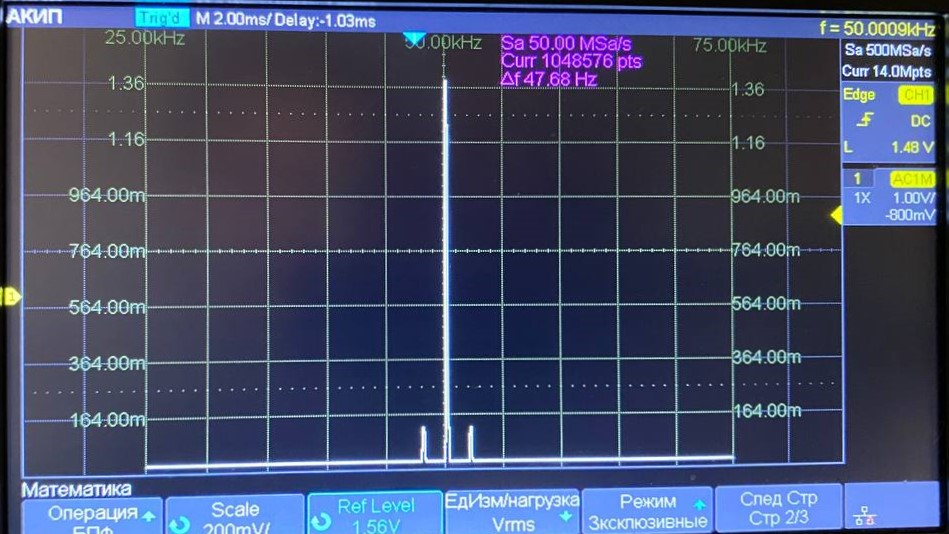
\includegraphics[width=0.9\textwidth]{photo_12.jpg}}}\\
 		\subfloat[$\nu_0 = 50$ кГц, $\nu_{\text{мод}} = 2$ кГц, $\phi_{m}$ = $20^\circ$.]{{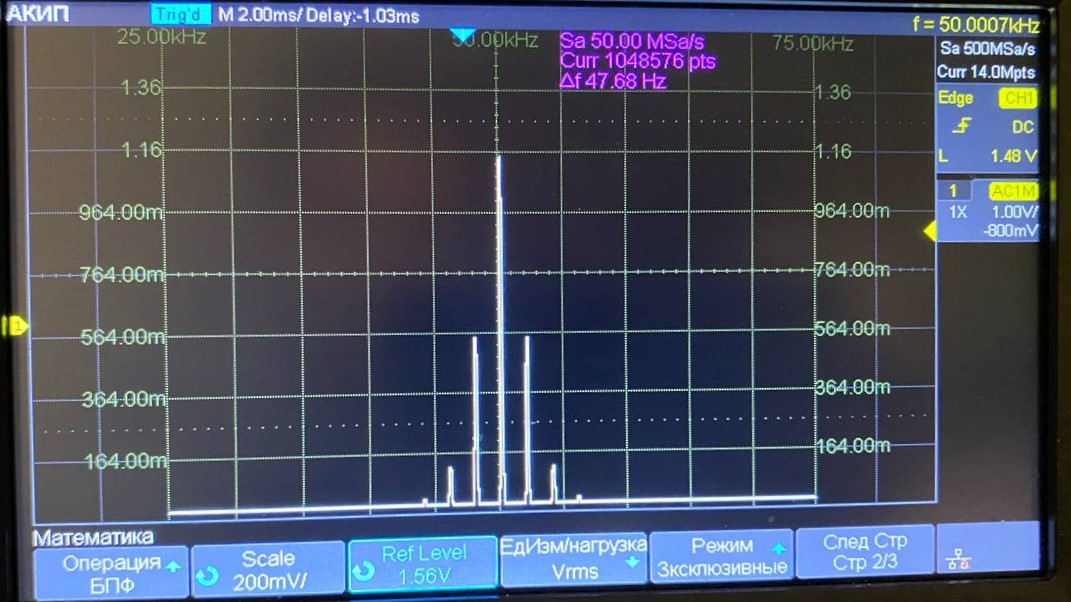
\includegraphics[width=0.478\textwidth]{photo_13.jpg}}}
 		\qquad
 		\subfloat[$\nu_0 = 50$ кГц, $\nu_{\text{мод}} = 2$ кГц, $\phi_{m}$ = $90^\circ$.]{{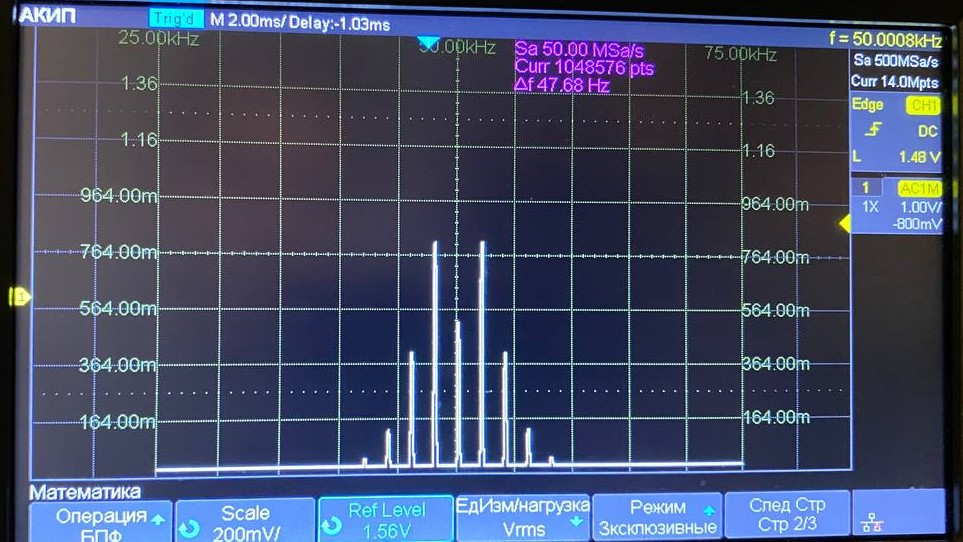
\includegraphics[width=0.478\textwidth]{photo_14.jpg}}}    		\caption{Спектр фазово модулированного сигнала}	
 	\end{figure}
 	\section{Выводы}
 	В ходе работы познакомились со спектром нескольких различных сигналов, изучили, как параметры характеризующие данные сигналы влияют на их спектры.\\
 	Для спектров прямоугольного сигнала, последовательности цугов, амплитудно модулированного сигнала проверили справедливость теоретических соотношений, характеризующих спектры.\\
 	Рассмотрели фазово модулированный сигнал и то, как на него влияет изменение фазы (изменение остальных параметров идентично амплитудно модулированному сигналу).
\end{document}